\documentclass[11pt,a4paper,titlepage]{article}
\usepackage[left=1.5cm,text={18cm, 25cm},top=2.5cm]{geometry}
\usepackage[utf8]{inputenc}
\usepackage{graphicx}
\usepackage[czech]{babel}
\usepackage{float}
\usepackage{color}
\usepackage{hyperref}
\usepackage{etoolbox}

\setlength{\parindent}{0cm}
\setlength{\parskip}{1em}
\sloppy

\hypersetup{
	colorlinks=true,
	linktoc=all,
	linkcolor=blue,
	citecolor=red,
	urlcolor=blue,
}

\begin{document}

		%\setstretch{0.5}
		\begin{center}

			
\includegraphics[width = 150mm]{img/logo.png}\\

			\vspace{\stretch{0.382}}

			\LARGE
			Získávání znalostí z databází\\
			Databáze ze sčítání lidu - zadání\\
			\vspace{\stretch{0.618}}

		\end{center}

	\Large{\today} \hfill Jiří Matějka, Lucie Pelantová
	\thispagestyle{empty}
	\newpage
	\setcounter{page}{1}

    \section{Úvod}
        Cílem tohoto projektu je získání zajímavých souvislostí z vybrané datové sady. Pro tento účel byla použita data ze sčítání lidu.
        
        Dolováním z této datové sady bude v rámci tohoto projektu zkoumán vliv zázemí občana na výběr jeho povolání. Vytyčené cíle tohoto projektu jsou blíže popsané v kapitole \ref{cile}.
    
    \section{Popis dat}
    Data ze sčítání lidu byla získána z databáze Census Bureau\footnote{http://www.census.gov/ftp/pub/DES/www/welcome.html}. Data extrahoval Berry Becker z databáze z roku 1994 a následně z nich pomocí sady podmínek (například omezení na věk občana)  vybral vypovýdající záznamy. Poprvé tyto data citoval Ron Kohavi v článku \textit{Scaling Up the Accuracy of Naive-Bayes Classifiers: a Decision-Tree Hybrid}.
    
        Datová sada se skládá ze 2 částí - soubor \textbf{adult.names} obsahuje popis jednotlivých údajů a soubor \textbf{adult.data} obsahuje samotná data.
    
    \section{Cíle projektu\label{cile}}
    
    Tento projekt si klade za cíle prozkoumání zajímavých souvislostí mezi zázemím občana a jeho volbou povolání. Při určování zázemí občana budou brány v potaz tyto údaje obsažené v datové sadě:
    
    \begin{itemize}
    	\item Věk
		\item Dosažené vzdělání
		\item Rodinný stav
		\item Role v rodině
		\item Rasová příslušnost
		\item Pohlaví
		\item Rodná země
    \end{itemize}
    
    
	Vliv na zvolené zaměstnání bude zkoumán ve dvou různých směrech:
    \begin{itemize}
        \item Pracovní třída - občan pracuje pod zaměstnavatelem, ve státním sektoru, jako osoba samostatně výdělečně činná, ...
        \item Povolání - občan pracuje například jako prodejce, poskytuje služby, v zemědělství, ...
    \end{itemize}

    \section{Předzpracování dat}
        V části předzpracování byl největší důraz kladen na číštění a redukci dat. Tímto procesem lze dosáhnout kvalitnější analýzi dat v následujících krocích. 
        
        \subsection{Čištění dat}
            Jak již bylo zmíněno v kapitole \ref{cile}, tento projekt je zaměřen na volbu povolání jednotlivých osob. Proto se v atributech týkajících se povolání (pracovní třída a povolání) doplňujeme chybějící hodnoty jejich predikcí. Predikce hodnot je prováděna za pomocí modelu, který byl vytrénovaný na použité datové sadě s použitím algoritmu k-NN.
        
        \subsection{Redukce dat}
            Redukce je dosažena pomocí snížení počtu dimenzí v datové sadě. Dimenze je snížena díky jednoduchému odstranění nerelevantních atributů, jako je například
            počet let studia či příjmy/výdaje z investic.
    
    \section{Získávání znalostí}
        V následující části projektu je množina dat rozdělena na trénovací a testovací sadu a to v poměru 7:3. Na jejichž základě je natrénovaný model, jehož přesnost je na zbývajích datech změřena. V rámci projektu bylo vyzkoušeno několik klasifikačních algoritmů, z níž některé pracují pouze s numerickými daty a proto bylo nutné pro samotnou klasifikaci použít operátor \textt{Nominal to Numerical}, kteý převede původní řetězcové hodnoty na numerické.

        \subsection{Klasifikační metody}
            První použitou metodou byl \textit{Naivní Bayesovský klasifikátor}. Jedná se o algoritmus, který dosahuje dobrých výsledků i při trénování na malé množině dat. Na použité datové sadě dosáhl přesnosti pouze XX.XX \%.
            
            \begin{figure}[H]
                \centering
                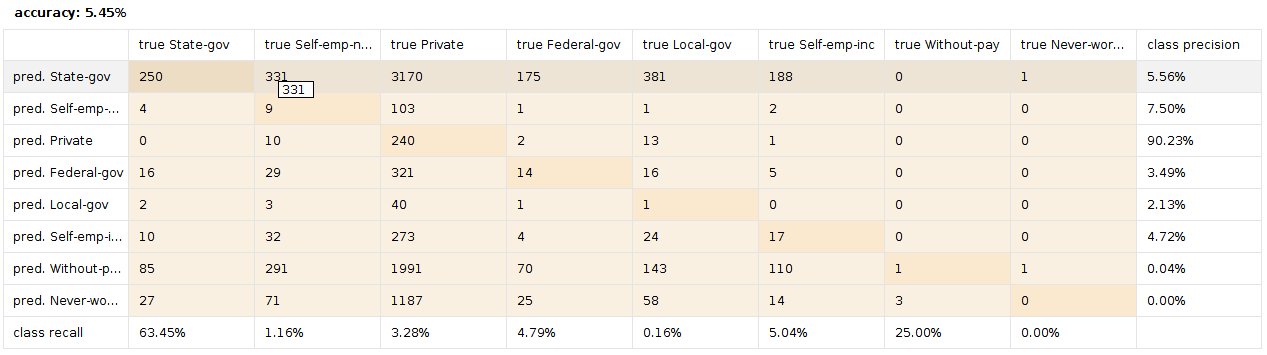
\includegraphics{./img/presnost_bayes.png}
                \caption{Výsledek predikce za použití metody \textit{Naivního Bayovského klasifikátoru}}
            \end{figure}

            Další použitou metodou byl \textit{Rozhodovací strom}. Jedná o algoritmus vhodný pro hledání skrytých závislostí v datech. Oproti předchozí metodě (\textit{Naivní Bayesovský klasifikátor}) bylo dosaženo nepatrného zlepšení. Výsledná přesnost tohoto modelu je XX.XX \%.
            
            \begin{figure}[H]
                \centering
                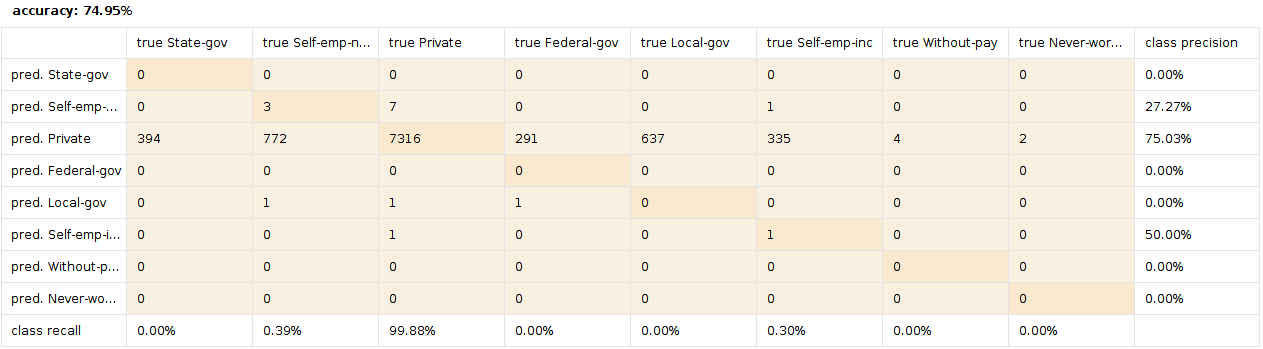
\includegraphics{./img/presnost_tree.png}
                \caption{Výsledek predikce za použití \textit{Rozhodovacího stromu}}
            \end{figure}

            Zajímavých výsledků bylo dosaženo pomocí \textit{Metody podpůrných vektorů}. Jedná se o často používanou metodu pro klasifikaci a regresní analýzu, protože dosahuje dobrých výsledků pro široké spektrum učících problémů.

            \begin{figure}[H]
                \centering
                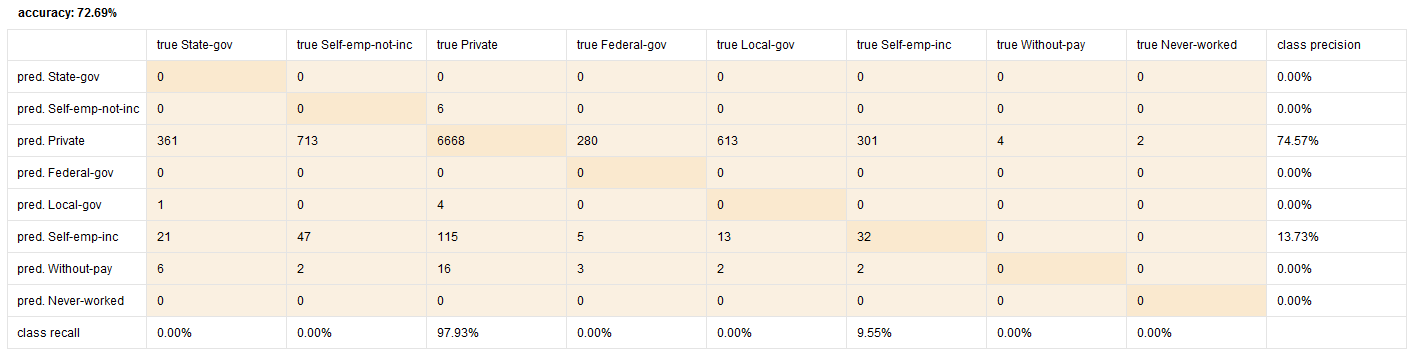
\includegraphics{./img/presnost_svm.png}
                \caption{Výsledek predikce za použití \textit{Metody podpůrných vektorů}}
            \end{figure}

            Z kategorie neuronových sítí byly použity metody \textit{Hluboké učení}, \textit{Neoronové sítě} a \textit{Perceprony}. Tyto metody dosáhly podobných výsledků jako rozhodovací strom a mezi sebou se liši v řádu desetin procent. Jejich přesnost se pohybovala okolo XX.XX \%.

            \begin{figure}[H]
                \centering
                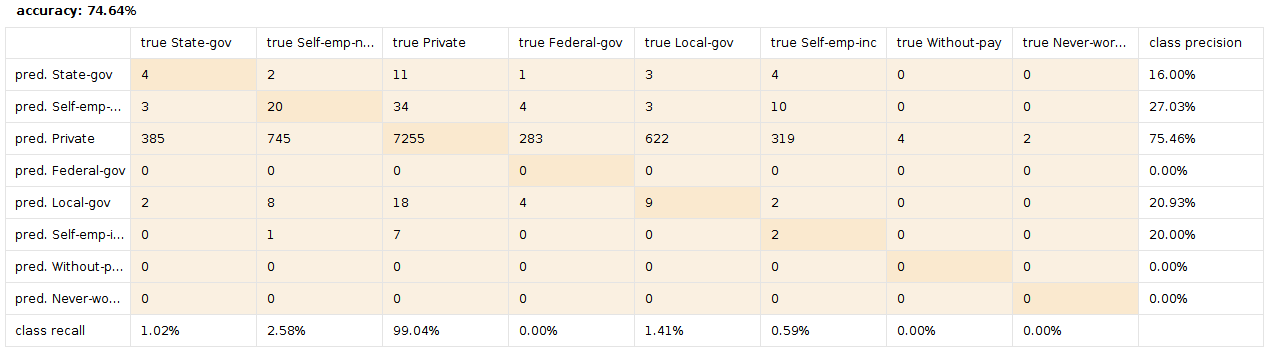
\includegraphics{./img/presnost_neural.png}
                \caption{Výsledek predikce za použití metody Naivního Bayovského klasifikátoru}
            \end{figure}

    \section{Výsledky}
        
        
    
\end{document}
